% شبکهٔ Ising: اسپین‌ها، جفت‌شدگی ZZ، میدان موضعی
% سبک مشترک نمودارهای سند پایه‌ها (فقط داخل محیط latin فراخوانی شود)
\tikzset{
	qafbox/.style={
		draw=black!55,
		rounded corners=2pt,
		align=center,
		inner sep=3pt,
		thick,
		fill=white,
		font=\footnotesize\linespread{1}\selectfont,
		minimum height=0.95cm
	},
	qafwide/.style={
		qafbox,
		text width=2.55cm
	},
	qafnarr/.style={
		qafbox,
		text width=2.05cm
	},
	qaftitle/.style={
		font=\small\bfseries\linespread{1}\selectfont,
		align=center
	},
	qafarr/.style={
		-{Latex[length=2.2mm]},
		thick,
		draw=black!65
	},
	qafpanel/.style={
		draw,
		thick,
		rounded corners=4pt,
		inner xsep=8pt,
		inner ysep=8pt
	}
}

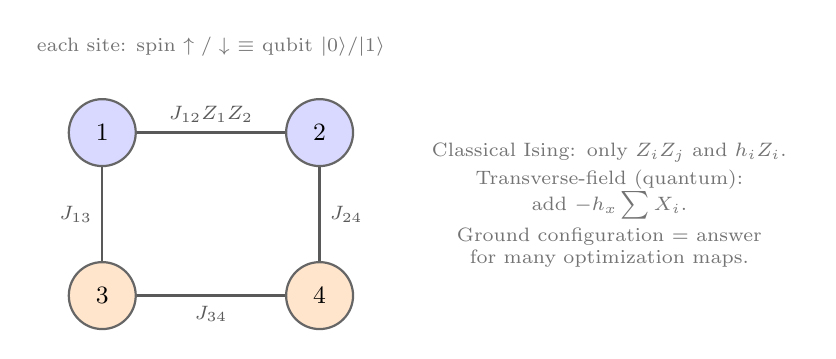
\begin{tikzpicture}[
	x=1.15cm,
	y=1.15cm,
	execute at begin picture={\hyphenpenalty=10000 \exhyphenpenalty=10000},
	spin/.style={circle, draw=black!60, thick, minimum size=0.85cm, inner sep=0pt, font=\small\bfseries},
	note/.style={font=\scriptsize, text=black!55, align=center}
	]
	\node[spin, fill=blue!15] (s1) at (0,1.2) {$1$};
	\node[spin, fill=blue!15] (s2) at (2.4,1.2) {$2$};
	\node[spin, fill=orange!20] (s3) at (0,-0.6) {$3$};
	\node[spin, fill=orange!20] (s4) at (2.4,-0.6) {$4$};

	\draw[thick, black!65] (s1) -- (s2) node[midway, above, font=\scriptsize] {$J_{12}Z_1Z_2$};
	\draw[thick, black!65] (s1) -- (s3) node[midway, left, font=\scriptsize] {$J_{13}$};
	\draw[thick, black!65] (s2) -- (s4) node[midway, right, font=\scriptsize] {$J_{24}$};
	\draw[thick, black!65] (s3) -- (s4) node[midway, below, font=\scriptsize] {$J_{34}$};

	\node[note] at (1.2,2.15) {each site: spin $\uparrow/\downarrow$ $\equiv$ qubit $|0\rangle/|1\rangle$};
	\node[note, text width=4.8cm] at (5.6,0.4) {%
		Classical Ising: only $Z_iZ_j$ and $h_i Z_i$.\\[2pt]
		Transverse-field (quantum): add $-h_x\sum X_i$.\\[2pt]
		Ground configuration $=$ answer for many optimization maps.};
\end{tikzpicture}
